\section{A direct local-energy construction}\label{sec:local-energy}

We now attack the single smoothed sum \(B\) of
Proposition~\ref{prop:smoothed}. The construction in this section
controls point evaluation by a neighboring-scale mean square without
assuming a zero-free half-plane. It then separates a computable
diagonal from the signed arithmetic term still requiring an estimate.
The results of this section do not establish that estimate.

\subsection{Reconstruction with a logarithmic cost}

For any complex sequence with \(|a_n|\le1\), put
\[
 F(X)=\sum_{n\ge1}a_ne^{-n/X},\qquad
 \mathcal H_F(X)=\int_{X/2}^{2X}|F(Y)|^2\frac{\dd Y}{Y}.
\]
Both expressions converge absolutely for \(X>0\).

\begin{theorem}[Explicit analytic localization]\label{thm:analytic-local}
For \(X\ge1\) and \(m=\lceil8\log_2(2X)\rceil\),
\begin{equation}\label{eq:analytic-local}
 |F(X)|^2\le10(m+2)\mathcal H_F(X)+X^{-4}.
\end{equation}
There is an explicit degree-\(m\) polynomial kernel \(K_m(0,u)\)
on \([-1/4,1/4]\) such that
\[
 F(X)=\int_{-1/4}^{1/4}K_m(0,u)
             F\!\left(\frac X{1+u}\right)\dd u+\mathcal R_X,
 \qquad
 |\mathcal R_X|\le\frac{\sqrt{2(m+2)}}{128X^7}.
\]
\end{theorem}
\begin{proof}
The holomorphic function
\[
 G_X(z)=\sum_{n\ge1}a_ne^{-n(1+z)/X}
\]
is defined for \(\operatorname{Re}z>-1\). On \(|z|\le1/2\),
\[
 |G_X(z)|\le(e^{1/(2X)}-1)^{-1}\le2X.
\]
Let \(P_m\) be its Taylor polynomial at zero. Cauchy's estimate gives
\[
 \sup_{|u|\le1/4}|G_X(u)-P_m(u)|
 \le2X\sum_{j>m}(2|u|)^j
 \le2X\,2^{-m}=:\delta.
\]
In particular \(P_m(0)=G_X(0)=F(X)\) exactly.

Let \(L_j\) denote the Legendre polynomial normalized by \(L_j(1)=1\).
Its norm on \([-1,1]\) is \(2/(2j+1)\). For completeness these
identities follow from Rodrigues' formula
\[
 L_j(t)=\frac1{2^j j!}\frac{\dd^j}{\dd t^j}(t^2-1)^j.
\]
Integration by parts \(j\) times proves orthogonality to polynomials
of degree less than \(j\). Its leading coefficient is
\((2j)!/(2^j(j!)^2)\); the recurrence
\(\int_{-1}^1(1-t^2)^j\dd t
 =\frac{2j}{2j+1}\int_{-1}^1(1-t^2)^{j-1}\dd t\)
then gives the stated norm.
Thus the evaluation kernel on the shorter interval is
\[
 K_m(0,u)=2\sum_{j=0}^m(2j+1)L_j(0)L_j(4u).
\]
Expanding a polynomial in this orthogonal basis gives
\begin{equation}\label{eq:kernel-reproduce}
 P(0)=\int_{-1/4}^{1/4}K_m(0,u)P(u)\dd u,\qquad
 |P(0)|^2\le K_m(0,0)\int_{-1/4}^{1/4}|P(u)|^2\dd u.
\end{equation}
These are classical reproducing-kernel identities
\cite[\S18.2(v)]{dlmf}; their constants have been derived here.
\footnote{The polynomial approximation is applied to the analytic
function of reciprocal scale, not to the arithmetic coefficients.
It therefore does not assume cancellation of \(\lambda\).}

Rodrigues' formula also gives
\[
 L_{2r+1}(0)=0,\quad
 L_{2r}(0)=(-1)^r\binom{2r}{r}4^{-r},\quad
 \left(\binom{2r}{r}4^{-r}\right)^2\le\frac1{r+1}.
\]
The last inequality follows by induction, since
\((2r+1)^2(r+2)\le4(r+1)^3\). Consequently
\[
 K_m(0,0)
 =2\sum_{r\le m/2}(4r+1)
      \left(\binom{2r}{r}4^{-r}\right)^2
 \le4(m+2).
\]
Apply \eqref{eq:kernel-reproduce} to \(P_m\) and use
\(|P_m|^2\le2|G_X|^2+2\delta^2\):
\[
 |F(X)|^2\le8(m+2)\int_{-1/4}^{1/4}|G_X(u)|^2\dd u
             +4(m+2)\delta^2.
\]
The substitution \(Y=X/(1+u)\) bounds this integral by
\[
 \int_{4X/5}^{4X/3}|F(Y)|^2\frac X{Y^2}\dd Y
 \le\frac54\mathcal H_F(X).
\]
Also \(\delta\le(128X^7)^{-1}\) and \(m+2\le16X\) for \(X\ge1\).
Hence \(4(m+2)\delta^2\le X^{-4}\), proving
\eqref{eq:analytic-local}. Finally
\(\int|K_m(0,u)|\dd u\le\sqrt{K_m(0,0)/2}\)
applied to \(G_X-P_m\) gives the reconstruction formula and error.
\end{proof}

In particular, \(\mathcal H_B(X)\ll_\varepsilon X^{1+\varepsilon}\)
would imply the requested pointwise square-root estimate. Only the
analytic transfer has been proved; it supplies no upper bound for
\(\mathcal H_B\).

\begin{figure}[ht]
\centering
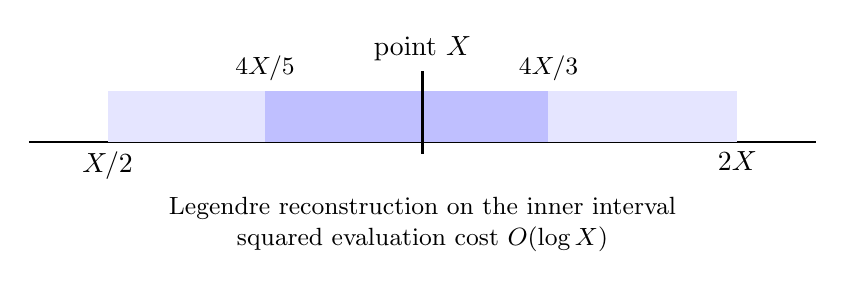
\begin{tikzpicture}[x=1cm,y=1cm]
 \draw[thick] (0,0)--(10,0);
 \fill[blue!10] (1,0) rectangle (9,.65);
 \fill[blue!25] (3,0) rectangle (6.6,.65);
 \draw[thick] (5,-.15)--(5,.9);
 \node[below] at (1,0) {\(X/2\)};
 \node[below] at (9,0) {\(2X\)};
 \node[above] at (5,.9) {point \(X\)};
 \node[above,font=\small] at (3,.65) {\(4X/5\)};
 \node[above,font=\small] at (6.6,.65) {\(4X/3\)};
 \node[align=center,font=\small] at (5,-1.05)
  {Legendre reconstruction on the inner interval\\
   squared evaluation cost \(O(\log X)\)};
\end{tikzpicture}
\caption{Localization in scale, shown schematically. The kernel
recovers the point from nearby values. Arithmetic cancellation is
still required in their mean square.}\label{fig:local-reconstruction}
\end{figure}

\subsection{The exact signed term}

Define the positive kernel
\[
 K(v)=\int_{1/2}^2e^{-v/t}\frac{\dd t}{t}
     =\int_{1/2}^2e^{-vu}\frac{\dd u}{u}.
\]
Absolute convergence gives
\begin{align}
 \mathcal H_B(X)&=\mathcal D(X)+\mathcal O(X),
       \label{eq:local-off-diagonal}\\
 \mathcal D(X)&=\int_{X/2}^{2X}
             \frac1{e^{2/Y}-1}\frac{\dd Y}{Y},\nonumber\\
 \mathcal O(X)&=2\sum_{h\ge1}\sum_{n\ge1}
    \lambda(n)\lambda(n+h)K((2n+h)/X).\nonumber
\end{align}
The symbol \(\mathcal O(X)\) in this display names a function,
not a big-\(O\) estimate.

\begin{proposition}[A diagonal with an explicit error]\label{prop:local-diagonal}
For every \(X>0\),
\[
 0<\mathcal D(X)-\left(\frac{3X}4-\log2\right)<\frac1{4X}.
\]
\end{proposition}
\begin{proof}
For \(t>0\),
\[
 0<\frac1{e^t-1}-\frac1t+\frac12<\frac t{12}.
\]
The lower inequality follows by differentiating
\((t-2)e^t+t+2\) twice. For the upper inequality, multiplication by
\(12t(e^t-1)\) reduces it to
\[
 (t^2-6t+12)(e^t-1)-12t
   =\sum_{j\ge5}\frac{(j-3)(j-4)}{j!}t^j>0.
\]
Substitute \(t=2/Y\) and integrate. The first two terms give
\(3X/4-\log2\), and the error is less than
\(\frac16\int_{X/2}^{2X}Y^{-2}\dd Y=1/(4X)\).
\end{proof}

Therefore a signed upper bound
\(\mathcal O(X)\ll_\varepsilon X^{1+\varepsilon}\)
would suffice. Replacing its terms by absolute values only gives
order \(X^2\). Positivity of \(\mathcal H_B\) gives a lower bound
for \(\mathcal O\), not the missing upper bound.

Complete multiplicativity reorganizes the same energy as
\[
 \mathcal H_B(X)=\sum_{k\ge2}c(k)
       \int_{X/2}^{2X}\frac1{e^{k/Y}-1}\frac{\dd Y}{Y},
 \qquad
 c(k)=\sum_{\substack{1\le a<k\\(a,k)=1}}
             \lambda(a)\lambda(k-a).
\]
Indeed write the two indices as \(da,db\) with \((a,b)=1\);
their signs multiply to \(\lambda(a)\lambda(b)\).
The term \(c(2)=1\) is exactly the diagonal. The remaining terms
are coprime additive correlations. The identity leaves their
cancellation to be proved.

\subsection{Why a prime Gram argument does not close the estimate}

The logarithmic identity obtained from complete multiplicativity is
\begin{align*}
 (\lambda\log)(n)&=(\lambda*(\lambda\Lambda))(n),\\
 \lambda(d)\Lambda(d)
   &=2\mathbf1_{d=\square}\Lambda(\sqrt d)-\Lambda(d).
\end{align*}
Checking prime powers proves the second line. Smoothing gives
\begin{equation}\label{eq:lambda-log-renewal}
 \sum_{n\ge1}\lambda(n)\log n\,e^{-n/X}
 =2\sum_{d\ge1}\Lambda(d)B(X/d^2)
     -\sum_{d\ge1}\Lambda(d)B(X/d).
\end{equation}
All sums converge absolutely at fixed \(X\).
However, for distinct primes \(p,q\),
\[
 \sum_{n\le N}\lambda(pn)\lambda(qn)=N.
\]
Thus prime dilations are maximally correlated in this Gram
calculation. Treating them as orthogonal would discard a full
off-diagonal. The identity \eqref{eq:lambda-log-renewal} is not a
contraction estimate.\footnote{Almost-all short-interval results
compare short and long averages \cite{mr-short}. That comparison
does not supply the square-root size of the long average required
here. We do not use a short-interval estimate with this additional
strength as an unstated premise.}

\subsection{An explicit finite-prime model}

Let \(f_y\) be completely multiplicative, equal to \(-1\) at primes
at most \(y\) and to \(+1\) at larger primes. Write
\[
 B_y(X)=\sum_{n\ge1}f_y(n)e^{-n/X},\qquad
 c_y=\prod_{p\le y}\frac{p-1}{p+1},\qquad
 G_y(\sigma)=\prod_{p\le y}
             \frac{1+p^{-\sigma}}{1-p^{-\sigma}}.
\]

\begin{theorem}[Finite-prime main term]\label{thm:finite-prime}
For \(X>0\), \(y\ge2\), and \(0<\sigma<1\),
\begin{equation}\label{eq:finite-prime}
 |B_y(X)-c_yX|\le X^\sigma G_y(\sigma).
\end{equation}
In particular, for \(y=(\log X)^2\) as \(X\to\infty\),
\[
 B_y(X)=c_yX+O(X^{1/2+o(1)}),\qquad
 B_y(X)\ge\frac{X}{2(\log X)^4}
\]
for all sufficiently large \(X\).
\end{theorem}
\begin{proof}
Define \(g_y\) multiplicatively by \(g_y(p^j)=2(-1)^j\)
for \(p\le y\), \(j\ge1\), and zero on powers of larger primes.
Prime by prime \(f_y=\mathbf1*g_y\). Hence
\[
 B_y(X)=\sum_{d\ge1}\frac{g_y(d)}{e^{d/X}-1},\quad
 \sum_{d\ge1}\frac{g_y(d)}d=c_y,\quad
 \sum_{d\ge1}\frac{|g_y(d)|}{d^\sigma}=G_y(\sigma).
\]
Only finitely many primes support \(g_y\), so these Dirichlet sums
converge absolutely for \(\sigma>0\). Also
\[
 0<\frac1t-\frac1{e^t-1}
 \le\min(1/2,1/t)\le t^{-\sigma}.
\]
Subtract \(X\sum g_y(d)/d\) and apply this term by term to obtain
\eqref{eq:finite-prime}.

The elementary Chebyshev bound gives
\(\pi(t)\ll t/\log t\), and partial summation then gives
\[
 \log G_y(1/2)\ll\sum_{p\le y}p^{-1/2}
                 \ll\frac{\sqrt y}{\log y}.
\]
The elementary details are recorded in Appendix~\ref{app:attack-checks}.
For \(y=(\log X)^2\), this is \(o(\log X)\), so
\(G_y(1/2)=X^{o(1)}\).
If \(r=\lfloor y\rfloor\), positivity of the factors gives
\[
 c_y\ge\prod_{n=2}^r\frac{n-1}{n+1}
      =\frac2{r(r+1)}\ge y^{-2}.
\]
The error \(X^{1/2+o(1)}\) is eventually less than
\(X/(2(\log X)^4)\), proving the last assertion.
\end{proof}

This is a bound for an explicitly constructed comparison function,
not for \(\lambda\). It shows that complete multiplicativity plus
agreement at all primes through \((\log X)^2\) cannot yield a
uniform square-root bound over the resulting class of functions.

\subsection{The large-prime cancellation that remains}

Put \(P^-(1)=\infty\), and define
\[
 h_y(d)=
 \begin{cases}
   2^{\omega(d)}\lambda(d),&P^-(d)>y,\\
   0,&\text{otherwise}.
 \end{cases}
\]
At a prime greater than \(y\), convolution by its local coefficients
\[
 1+2\sum_{j\ge1}(-1)^jp^{-js}
       =\frac{1-p^{-s}}{1+p^{-s}}
\]
changes the local signs of \(f_y\) to those of \(\lambda\).
Therefore \(\lambda=f_y*h_y\), and
\begin{equation}\label{eq:prime-tail-exact}
 B(X)=B_y(X)+T_y(X),\qquad
 T_y(X)=\sum_{\substack{d>1\\P^-(d)>y}}
                h_y(d)B_y(X/d).
\end{equation}
Exponential decay justifies this identity absolutely at every
fixed \(X\). With \(y=(\log X)^2\), the desired estimate would follow
from
\begin{equation}\label{eq:prime-tail-target}
 T_y(X)=-c_yX+O_\varepsilon(X^{1/2+\varepsilon}).
\end{equation}
The comparison-kernel error in Theorem~\ref{thm:finite-prime}
is already of square-root size with a subpower loss.
The signed estimate \eqref{eq:prime-tail-target} remains unproved.

% Proof-ready insertion after eq:prime-tail-target in local-energy.tex.
% Uses the classical Davenport estimate already invoked in sec:sieve.
\begin{proposition}[Prime-tail cancellation to logarithmic order]
\label{prop:prime-tail-logarithmic}
For \(y=(\log X)^2\), and every fixed \(A>0\),
\[
 T_y(X)=-c_yX+O_A\!\left(\frac{X}{(\log X)^A}\right).
\]
In particular, \(T_y(X)/(c_yX)\to-1\).
\end{proposition}
\begin{proof}
The classical uniform additive estimate of Davenport, in the
Liouville form recalled in Section~\ref{sec:sieve} and quoted in
\cite{mrt}, gives at additive frequency zero
\[
 L(t)\ll_A \frac{t}{(\log(2t))^A}
 \qquad(t\ge1).
\]
Partial summation gives the absolutely convergent identity
\[
 B(X)=\frac1X\int_1^\infty L(t)e^{-t/X}\dd t.
\]
For \(X\ge4\), the contribution from \(1\le t\le\sqrt X\)
has modulus at most \(X^{-1}\int_1^{\sqrt X}t\dd t\le1/2\).
For \(t\ge\sqrt X\), use
\(\log(2t)\ge\tfrac12\log X\) to bound the remaining part by
\[
 \frac{C_A2^A}{X(\log X)^A}
     \int_0^\infty te^{-t/X}\dd t
 =\frac{C_A2^AX}{(\log X)^A}.
\]
Consequently \(B(X)\ll_A X/(\log X)^A\).
By Theorem~\ref{thm:finite-prime} and
\eqref{eq:prime-tail-exact},
\[
 T_y(X)+c_yX
   =B(X)-\bigl(B_y(X)-c_yX\bigr)
   =O_A\!\left(\frac{X}{(\log X)^A}\right)
        +O(X^{1/2+o(1)}).
\]
For each fixed \(A\), the last error is absorbed in the first.
Finally \(c_y\ge(\log X)^{-4}\) gives
\(T_y(X)/(c_yX)=-1+O_A((\log X)^{4-A})\).
Take any \(A>4\).
\end{proof}

This proves the main-term cancellation in the actual exponential
kernel. It is a consequence of classical additive cancellation,
not a new zero-free theorem. Its error is larger than the
square-root error requested in \eqref{eq:prime-tail-target}.

\begin{proposition}[The precise power-saving endpoint]
\label{prop:prime-tail-rh-equivalence}
For \(y=(\log X)^2\), the estimate
\[
 T_y(X)+c_yX\ll_\varepsilon X^{1/2+\varepsilon}
 \quad\text{for every }\varepsilon>0
\]
is equivalent to RH.
\end{proposition}
\begin{proof}
The exact identity and Theorem~\ref{thm:finite-prime} give
\[
 T_y(X)+c_yX-B(X)=O(X^{1/2+o(1)}).
\]
Hence the asserted family of bounds holds if and only if
\(B(X)\ll_\varepsilon X^{1/2+\varepsilon}\) for every
\(\varepsilon>0\). The equivalence of the latter condition
with RH is Proposition~\ref{prop:smoothed}.
\end{proof}


There is a cancellation theorem in a different, convergent weight.
For real \(s>1\), Euler products give
\begin{equation}\label{eq:prime-tail-abel}
 H_y(s):=\sum_{d\ge1}\frac{h_y(d)}{d^s}
 =\frac{\zeta(2s)}{\zeta(s)^2c_y(s)},\qquad
 c_y(s)=\prod_{p\le y}\frac{1-p^{-s}}{1+p^{-s}}.
\end{equation}
Uniformly for \(0<\delta\le\delta_0\) and
\(\delta\log y\le1\),
\begin{equation}\label{eq:prime-tail-double-zero}
 H_y(1+\delta)
 =\frac{\zeta(2)\delta^2}{c_y}
       \left(1+O(\delta(1+\log y))\right).
\end{equation}
Indeed the pole of \(\zeta\) at one gives
\(\zeta(2+2\delta)/\zeta(1+\delta)^2
=\zeta(2)\delta^2(1+O(\delta))\), while
\[
 \frac{\dd}{\dd s}\log c_y(s)
 =2\sum_{p\le y}\frac{(\log p)p^{-s}}{1-p^{-2s}}
 \ll\log y\quad(s\ge1)
\]
by Chebyshev and partial summation. Integrating this derivative
proves the uniform factor in \eqref{eq:prime-tail-double-zero}.
For fixed \(y\), the tail without \(d=1\) tends to \(-1\).
This is an actual all-prime cancellation in the Abel weight.

The distinction between the two kernels is essential.
\footnote{The positive absolute-coefficient series is
\(\sum |h_y(d)|d^{-s}=\zeta(s)^2c_y(s)/\zeta(2s)\);
for fixed \(y\) it has a double pole at one. Thus absolute
comparison does not preserve the small signed value in
\eqref{eq:prime-tail-double-zero}.}
Equation \eqref{eq:prime-tail-double-zero} concerns
\(d^{-1-\delta}\), whereas \eqref{eq:prime-tail-exact} contains
the scale-dependent kernel \(B_y(X/d)\). No bound for their signed
discrepancy has been obtained. Treating their cancellation as
interchangeable would assume the unresolved step.

% Suitable following the existing Abel double-zero discussion.
For clarity, the double zero in \eqref{eq:prime-tail-double-zero}
does not exclude nonreal poles. For fixed \(y\), each finite
Euler factor of \(c_y(s)\) is holomorphic and nonzero on
\(\operatorname{Re}s>0\). If \(\rho\) were a zeta zero of
order \(r\) with \(\operatorname{Re}\rho>1/2\), then
\eqref{eq:prime-tail-abel} would have the leading Laurent term
\[
 H_y(s)=
 \frac{(r!)^2\zeta(2\rho)}
      {c_y(\rho)(\zeta^{(r)}(\rho))^2}
       (s-\rho)^{-2r}
       +O((s-\rho)^{1-2r}).
\]
The coefficient is nonzero. The local cancellation at one
therefore supplies no contradiction to such a zero; excluding
it requires the global power-saving estimate.
